\documentclass[11pt,a4paper]{article}

\usepackage[utf8]{inputenc}
\usepackage[T1]{fontenc}
\usepackage[english]{babel}
\usepackage{lmodern}
\usepackage[margin=2.5cm]{geometry}
\usepackage{booktabs}
\usepackage{longtable}
\usepackage{array}
\usepackage{enumitem}
\usepackage{xcolor}
\usepackage{tikz}
\usetikzlibrary{positioning, arrows.meta, fit}
\usepackage{caption}
\usepackage{hyperref}
\hypersetup{
  colorlinks = true,
  linkcolor  = blue!50!black,
  urlcolor   = blue!50!black,
  citecolor  = green!35!black,
  pdftitle   = {RAG Systems for Regulatory and Technical Documentation: Architectural Decision and MCP-Based Local RAG Server Proposal},
  pdfauthor  = {RAG Research Team}
}

\title{\textbf{RAG Systems for Regulatory and Technical Documentation}\\[2mm]
\large Architectural Decision Report and Proposal for a MCP-Based Local RAG Server}
\author{RAG Research Team\\Universidad Nacional de Colombia}
\date{\today}

\begin{document}

\maketitle

\begin{abstract}
\noindent
This report is a strategic evaluation framework for deciding what kind of
retrieval-augmented generation (RAG) architecture to build for regulatory and
technical documentation. It reviews the state of the art as of August 2026 --
native multimodal document parsing, hybrid retrieval combined with knowledge
graphs, and the emergence of the Model Context Protocol (MCP) as the standard
for context servers -- and compares two architectural paradigms (custom RAG
pipeline versus MCP-based RAG server) and two infrastructure paradigms (local
versus API/cloud deployment). Following this evaluation, the report proposes a
\textbf{MCP-based local RAG server} as the baseline architecture for a
controlled experimental comparison between local and API-based
implementations, and details the benchmarking methodology that this
architecture enables.
\end{abstract}

\section{Introduction}

\subsection{Purpose and Scope}

The purpose of this document is to provide the decision criteria needed to
choose the RAG architecture for a knowledge system built around complex
documents: regulations, technical documentation, hierarchies, and design
diagrams. It is explicitly \emph{not} an implementation guide. It evaluates
current industry philosophies (state of the art, 2026), the available tool
ecosystem, the complexity level of each alternative, and the user profile for
which each alternative is the best fit.

The report is organized in two parts. The first part (Sections~\ref{sec:sota}
to~\ref{sec:decision}) synthesizes the architectural decision guide. The
second part (Sections~\ref{sec:solution} to~\ref{sec:conclusions}) develops
the selected solution: a local RAG system exposed as an MCP server, together
with the experimental methodology proposed to benchmark it.

\section{State of the Art and Industry Trends (2026)}
\label{sec:sota}

Extracting knowledge from complex PDFs (regulations, hierarchies, design
diagrams) has moved beyond simple text chunking. Three trends define the
current landscape.

\subsection{Document Processing (SOTA Parsing)}

The industry has shifted toward \textbf{native multimodal models and semantic
parsers} (e.g., LlamaParse, Docling \cite{docling}) that understand tables and
complex structures without losing formatting. Parsing quality is now treated
as a first-class stage of the RAG pipeline rather than an incidental step.

\subsection{Hybrid Retrieval and GraphRAG}

Vector similarity alone is no longer the standard. Current solutions
\textbf{combine keyword search, dense vectors, and knowledge graphs}
\cite{graphrag} to connect regulatory articles that reference each other, so
that retrieval can follow both semantic proximity and explicit document
relations.

\subsection{Context Standardization}

The emergence of the \textbf{Model Context Protocol (MCP)}
\cite{mcp-spec,mcp-sdk} has changed the paradigm: instead of building
monolithic RAG applications, the trend is to create \emph{context servers}
connectable to any AI client or agent. This report adopts MCP as the
interoperability layer of the proposed solution.

\subsection{Evaluation Landscape}

Alongside these trends, the evaluation tooling has matured: RAG-specific
frameworks such as RAGAs \cite{ragas} and RAGChecker \cite{ragchecker},
embedding benchmarks (MTEB \cite{mteb}), vector database benchmarks
\cite{vdbbench}, local inference benchmarks \cite{localbench}, and general RAG
evaluation surveys \cite{rag-survey} provide the methodological basis for the
experimental design in Section~\ref{sec:methodology}. For visual-document
retrieval, ColPali \cite{colpali} represents the current research direction,
though it is out of scope for the initial prototype.

\section{Architecture Paradigm: Custom RAG vs. MCP Server}
\label{sec:architecture}

This section evaluates how to structure the solution at the software level.

\subsection{Custom RAG (Ad-Hoc Pipeline)}

A custom RAG builds the entire flow from scratch: ingestion, vector database,
retrieval, LLM orchestration, and frontend. It offers absolute control and
extreme optimization for highly specific workflows, but carries high
maintenance cost, a slow development cycle (months), and the risk of
``reinventing the wheel'' for integrations. It is the right choice for
AI-core products that need their own UI, highly specific re-ranking logic, or
deep integration with non-standard legacy systems.

\subsection{RAG Server via MCP}

An MCP-based RAG server packages the retrieval system (documents and
regulations) as a server that exposes its capabilities under the MCP
standard, allowing any MCP-compatible AI client to consume it. The philosophy
is ``write the context once, consume it anywhere''. Orchestration and
frontend are delegated to existing AI clients, which makes deployment
extremely fast (days to weeks) at the cost of functional dependency on the
client tool and less control over the final prompt and UI.

Table~\ref{tab:arch} summarizes both paradigms.

\begin{table}[htbp]
\centering
\begingroup
\footnotesize
\setlength{\tabcolsep}{4pt}
\begin{tabular}{>{\raggedright\arraybackslash}p{2.0cm}>{\raggedright\arraybackslash}p{6.4cm}>{\raggedright\arraybackslash}p{6.4cm}}
\toprule
\textbf{Attribute} & \textbf{Custom RAG (Ad-Hoc Pipeline)} & \textbf{RAG Server via MCP} \\
\midrule
Philosophy & Absolute control and extreme optimization for highly specific workflows. & ``Write the context once, consume it anywhere.'' Interoperability and open ecosystem. \\
Complexity & High. Requires constant pipeline maintenance and infrastructure management. & Medium/Low. Orchestration and frontend are delegated to existing AI clients. \\
Target user & Companies with AI-core products that need their own user interfaces, highly specific re-ranking logic, or deep integration with non-standard legacy systems. & Internal teams, design studios, or law firms that already use third-party AI assistants and only need to connect their private data without building a new application from scratch. \\
Advantages & Total flexibility, frontend customization, millisecond-level latency optimization. & Ultra-fast deployment (days/weeks), zero effort building user interfaces, native integration with developer and analyst workflows. \\
Disadvantages & High technical debt, slow development cycle (months), ``reinventing the wheel'' for integrations. & Functional dependency on the client tool (if the AI client reasons poorly, the RAG will fail); less control over the final prompt or the UI. \\
Ready-made tools & LangChain, LlamaIndex, Haystack, Qdrant/Pinecone, Streamlit/Vercel (for UI). & Official MCP SDKs, Smithery.ai (server registry). \\
Compatibility & Closed. Only communicates with the systems the development team explicitly programs. & Open and universal with SOTA clients: Claude Desktop, Cursor, Windsurf, Zed, and any MCP-compatible AI agent. \\
\bottomrule
\end{tabular}
\endgroup
\caption{Architectural paradigms: custom RAG pipeline versus RAG server via MCP.}
\label{tab:arch}
\end{table}

\section{Infrastructure Paradigm: Local vs. API (Cloud)}
\label{sec:infra}

This section evaluates where and how the AI models are processed and where
the data is stored.

\subsection{Local Deployment (On-Premise / Edge)}

Local deployment runs the embedding and generation models on company-owned
hardware. It is the target choice for government entities, law firms, defense,
or healthcare organizations with strict privacy regulations (HIPAA, strict
GDPR). It guarantees absolute privacy, fixed long-term cost, and immunity to
internet outages and provider rate limits. Its weaknesses are the VRAM
bottleneck when scaling to concurrent users and the lower reasoning capacity
of local models (7B--70B parameters) on complex legal or regulatory jargon.
Typical tools are Ollama, vLLM, LM Studio, llama.cpp, and HuggingFace TEI.

\subsection{API / Cloud (SaaS)}

API-based deployment consumes foundation models hosted by third parties
(OpenAI, Anthropic, Google, etc.). It is the target choice for startups,
agile companies, and teams that prioritize response quality and delivery
speed. It provides state-of-the-art reasoning, near-infinite scalability, and
optimized time-to-first-token latency. Its risks are cost leaks on long
documents, provider dependency, and legal or compliance barriers when
regulation forbids sending data to public clouds. Typical tools are the
OpenAI API, Anthropic API, Google Vertex AI, and AWS Bedrock.

Table~\ref{tab:infra} summarizes both paradigms.

\begin{table}[htbp]
\centering
\begingroup
\footnotesize
\setlength{\tabcolsep}{4pt}
\begin{tabular}{>{\raggedright\arraybackslash}p{2.0cm}>{\raggedright\arraybackslash}p{6.4cm}>{\raggedright\arraybackslash}p{6.4cm}}
\toprule
\textbf{Attribute} & \textbf{Local Deployment (On-Premise / Edge)} & \textbf{API / Cloud (SaaS)} \\
\midrule
Target user & Government entities, law firms, defense, or healthcare companies with strict privacy regulations (HIPAA, strict GDPR). & Startups, agile companies, and teams that prioritize response quality and delivery speed over data concerns (provided B2B no-training agreements are signed). \\
Complexity & Very High. Requires a DevOps/MLOps profile and costly hardware. & Low. The provider manages the hardware. \\
Advantages &
\begin{itemize}[leftmargin=1.2em, nosep, topsep=0pt]
  \item Absolute privacy: regulatory data and design secrets never leave the machine.
  \item Fixed long-term cost (no per-token payment).
  \item Immunity to internet outages and provider rate limits.
\end{itemize} &
\begin{itemize}[leftmargin=1.2em, nosep, topsep=0pt]
  \item Absolute state-of-the-art reasoning (2026 reasoning models, huge context windows).
  \item Infinite scalability: supports spikes of 1,000 users without extra configuration.
  \item Highly optimized time-to-first-token (TTFT) latency.
\end{itemize} \\
Disadvantages / where it breaks &
\begin{itemize}[leftmargin=1.2em, nosep, topsep=0pt]
  \item VRAM is the bottleneck: scaling to multiple concurrent users quickly brings the machine down.
  \item Less capable models: local LLMs (7B--70B parameters) often fail to match the deep reasoning required for complex legal/regulatory jargon compared with cloud models.
\end{itemize} &
\begin{itemize}[leftmargin=1.2em, nosep, topsep=0pt]
  \item Cost leaks: if the regulations are very long and the RAG is inefficient, the bill for millions of tokens can skyrocket.
  \item Provider dependency: global API outages affect the service.
  \item Legal/compliance barriers if regulation explicitly forbids sending data to public clouds.
\end{itemize} \\
Ready-made tools & Ollama, vLLM, LM Studio, llama.cpp, HuggingFace TEI. & OpenAI API, Anthropic API, Google Vertex AI, AWS Bedrock. \\
\bottomrule
\end{tabular}
\endgroup
\caption{Infrastructure paradigms: local versus API/cloud deployment.}
\label{tab:infra}
\end{table}

\section{Decision-Making Summary}
\label{sec:decision}

Table~\ref{tab:decision} summarizes the recommended architecture and
infrastructure per business scenario.

\begin{table}[htbp]
\centering
\begingroup
\footnotesize
\setlength{\tabcolsep}{4pt}
\begin{tabular}{>{\raggedright\arraybackslash}p{4.8cm}>{\raggedright\arraybackslash}p{4.8cm}>{\raggedright\arraybackslash}p{4.8cm}}
\toprule
\textbf{Business Scenario} & \textbf{Architectural Recommendation} & \textbf{Infrastructure Recommendation} \\
\midrule
Internal legal audit: a team reviews confidential regulations that cannot leave the network by law. They already use local assistants. & MCP Server RAG (to connect to their existing assistants). & Local (Ollama/vLLM) to guarantee total privacy. \\
B2B SaaS product: they want to sell their own web platform to architects for consulting building regulations. & Custom RAG (they need their own UI, analytics, and flow control). & API / Cloud to scale users quickly and use SOTA models. \\
Developer/designer productivity: the team needs technical design clarifications directly from their IDE (e.g., Cursor). & MCP Server RAG (integrates natively into their daily work environment). & API / Cloud (assuming the data is not government top-secret). \\
\bottomrule
\end{tabular}
\endgroup
\caption{Decision-making summary per business scenario.}
\label{tab:decision}
\end{table}

\section{Proposed Solution: MCP-Based Local RAG Server}
\label{sec:solution}

\subsection{Overview}

The selected solution uses a \textbf{Model Context Protocol (MCP) server} as
the standard interface between an LLM-based client and a fully local
Retrieval-Augmented Generation system. The key idea is that MCP is not the
RAG system itself: \textbf{MCP provides a standardized tool interface through
which an LLM can access the RAG system}.

The architecture separates three concerns:

\begin{enumerate}[leftmargin=1.6em]
  \item \textbf{Knowledge layer} --- documents, embeddings, and vector storage.
  \item \textbf{Retrieval layer} --- semantic search over the local knowledge base.
  \item \textbf{Interaction layer} --- an MCP server exposing retrieval capabilities as tools to compatible clients.
\end{enumerate}

This separation makes the solution particularly suitable for an experimental
comparison between \textbf{local execution} and \textbf{API-based approaches}.

\subsection{Interaction Flow}

Conceptually, the MCP server acts as a controlled bridge between an LLM
client and the local knowledge base. Figure~\ref{fig:flow} shows the typical
flow.

\begin{figure}[htbp]
\centering
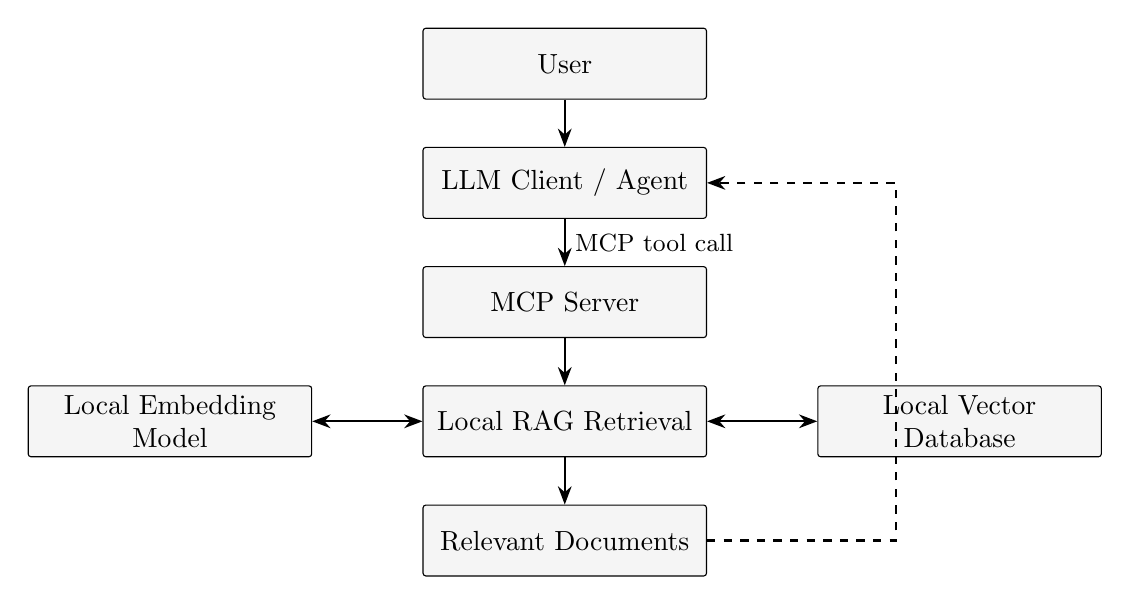
\begin{tikzpicture}[
    box/.style={draw, rounded corners=1pt, align=center,
                minimum width=36mm, minimum height=9mm, fill=gray!8},
    arr/.style={-{Stealth}, thick},
    bi/.style={{Stealth}-{Stealth}, thick}
  ]
  \node[box] (user)   {User};
  \node[box, below=6mm of user]  (client) {LLM Client / Agent};
  \node[box, below=6mm of client] (mcp)    {MCP Server};
  \node[box, below=6mm of mcp]   (rag)    {Local RAG Retrieval};
  \node[box, left=14mm of rag]   (emb)    {Local Embedding\\Model};
  \node[box, right=14mm of rag]  (vdb)    {Local Vector\\Database};
  \node[box, below=6mm of rag]   (docs)   {Relevant Documents};

  \draw[arr] (user)   -- (client);
  \draw[arr] (client) -- node[right, font=\small] {MCP tool call} (mcp);
  \draw[arr] (mcp)    -- (rag);
  \draw[bi]  (rag)    -- (emb);
  \draw[bi]  (rag)    -- (vdb);
  \draw[arr] (rag)    -- (docs);
  \draw[arr, dashed] (docs.east) -- ++(24mm,0) |- (client.east);
\end{tikzpicture}
\caption{Typical interaction flow between the user, the LLM client, the MCP server, and the local RAG retrieval system.}
\label{fig:flow}
\end{figure}

The MCP server does not need to contain the LLM itself. Its responsibility is
to expose well-defined capabilities, such as:

\begin{itemize}[leftmargin=1.6em]
  \item Searching the local knowledge base.
  \item Retrieving relevant document fragments.
  \item Potentially listing available documents.
  \item Potentially retrieving metadata or document information.
  \item Providing a consistent interface for future RAG operations.
\end{itemize}

The LLM decides \textbf{when} to use the retrieval tool, while the MCP server
controls \textbf{how} the retrieval operation is performed.

\subsection{Why MCP Is a Good Architectural Choice}

Without MCP, an application needs a custom interface between the LLM and the
RAG system. With MCP, the RAG capability is exposed through a \textbf{standard
protocol instead of a client-specific integration}. This reduces the amount
of interface code that has to be maintained and makes the RAG server easier
to reuse with different MCP-compatible clients.

\subsection{Methodological Rationale}

The strongest reason to use MCP in this project is methodological rather than
purely technical: the objective is to evaluate different ways of providing an
LLM with access to knowledge while keeping the underlying retrieval
capability as consistent as possible.

An MCP-based architecture establishes a clear experimental boundary
(Figure~\ref{fig:boundary}), so the client and the server can be treated as
separate experimental components.

\begin{figure}[htbp]
\centering
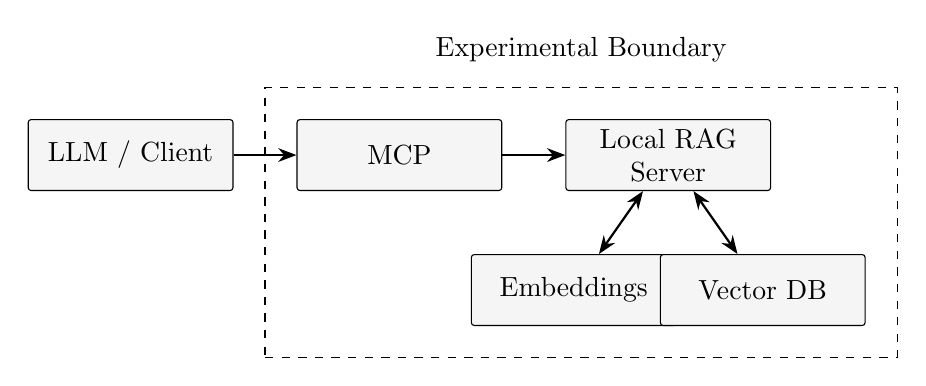
\begin{tikzpicture}[
    box/.style={draw, rounded corners=1pt, align=center,
                minimum width=26mm, minimum height=9mm, fill=gray!8},
    arr/.style={-{Stealth}, thick},
    bi/.style={{Stealth}-{Stealth}, thick}
  ]
  \node[box] (client) {LLM / Client};
  \node[box, right=8mm of client] (mcp) {MCP};
  \node[box, right=8mm of mcp] (server) {Local RAG\\Server};
  \node[box, below=8mm of server, xshift=-12mm] (emb) {Embeddings};
  \node[box, below=8mm of server, xshift=12mm] (vdb) {Vector DB};
  \node[draw, dashed, fit=(mcp)(server)(emb)(vdb), inner sep=4mm,
        label={[above=2mm]Experimental Boundary}] {};

  \draw[arr] (client) -- (mcp);
  \draw[arr] (mcp)    -- (server);
  \draw[bi]  (server) -- (emb);
  \draw[bi]  (server) -- (vdb);
\end{tikzpicture}
\caption{The MCP interface defines the experimental boundary between the LLM client and the local RAG implementation.}
\label{fig:boundary}
\end{figure}

This design makes it easier to compare variables such as: local versus
API-based embeddings; local versus cloud-based retrieval infrastructure;
retrieval latency; end-to-end response latency; CPU utilization; RAM
consumption; storage requirements; network dependency; retrieval quality; and
operational complexity.

Most importantly, the \textbf{retrieval interface can remain stable while the
implementation behind it changes}. The same MCP tool
(\texttt{search\_knowledge\_base(query)}) can remain in place while the
underlying implementation changes from \emph{local embeddings + local vector
database} to \emph{API embeddings + remote vector database}. This makes the
comparison cleaner because the interface exposed to the LLM does not change.

\subsection{Advantages}

\begin{itemize}[leftmargin=1.6em]
  \item \textbf{Separation of concerns.} The LLM does not need to know which embedding model, vector database, or storage layout is used, or how similarity search and indexing are implemented.
  \item \textbf{Reusability.} A single MCP server can be consumed by multiple compatible clients (CLI agent, desktop client, other MCP clients) without rewriting the RAG implementation.
  \item \textbf{Local execution.} Documents, embedding model, vector database, retrieval logic, and the MCP server can all stay on the user's machine, minimizing external dependencies and network traffic.
  \item \textbf{Easy substitution of components.} Embedding models (e.g., all-MiniLM-L6-v2, other local models, API-based models) and vector stores (ChromaDB, other local databases, remote databases) can be replaced independently while the MCP interface remains approximately the same.
  \item \textbf{Good fit for benchmarking.} The server provides a defined boundary from which the RAG subsystem can be measured independently (embedding time, indexing time, retrieval latency, memory and CPU usage, storage, retrieval relevance).
  \item \textbf{Low implementation complexity.} A basic prototype only requires: initialize the MCP server, initialize the local embedding model, initialize the vector database, load/index documents, expose the search operation as an MCP tool, and wait for client requests. No custom protocol, API gateway, or client-specific integration is needed.
\end{itemize}

\subsection{Disadvantages and Limitations}

\begin{itemize}[leftmargin=1.6em]
  \item \textbf{MCP adds an integration layer.} If the only requirement is a simple local application performing retrieval, a direct function call is simpler. MCP should be justified by interoperability, tool-based LLM interaction, or architectural separation.
  \item \textbf{Client compatibility.} The benefits depend on the availability of MCP-compatible clients; a conventional application cannot consume an MCP server without an adapter.
  \item \textbf{Process and communication overhead.} A separate MCP process communicating over standard input/output adds overhead relative to a direct function call, which should be considered in precise latency measurements.
  \item \textbf{MCP does not solve RAG quality.} It standardizes access to tools but does not guarantee good chunking, embeddings, retrieval quality, ranking, parsing, citations, or generated answers.
  \item \textbf{Local does not mean resource-free.} Indexing can still consume significant CPU, RAM, disk space, and processing time; model selection and indexing strategy are experimental variables for larger collections.
\end{itemize}

\section{Proposed Experimental Methodology}
\label{sec:methodology}

For a meaningful comparison, the system must use the \textbf{same document
collection and evaluation questions} across the different implementations
(local and API-based).

\subsection{Phase 1 --- Dataset Preparation}

Prepare a controlled, \emph{versioned} document collection containing
representative material: PDF documents, technical documentation, plain-text
files, source-code repositories, markdown documentation, and standards or
regulatory documents. For the Colombian regulatory domain, the ANE/MinTIC
compilation \cite{ane-mintic} is a concrete candidate corpus. Versioning
guarantees every experiment uses the same source material.

\subsection{Phase 2 --- Local Indexing}

Process the documents with a reproducible pipeline:
\texttt{text extraction} $\rightarrow$ \texttt{chunking} $\rightarrow$
\texttt{embedding generation} $\rightarrow$ \texttt{vector index}. Record the
number of documents, number of chunks, total text size, indexing time,
embedding generation time, and storage size. Document ingestion and retrieval
must be treated as separate stages: ingestion creates the searchable
knowledge base once, and the MCP tool performs retrieval at query time.

\subsection{Phase 3 --- MCP Exposure}

Expose retrieval through a small number of well-defined MCP tools, e.g.,
\texttt{search\_knowledge\_base(query, top\_k)}. The tool should return enough
information for the LLM to understand the retrieved context, ideally including
document identifiers or metadata.

\subsection{Phase 4 --- Controlled Queries}

Create a fixed benchmark set of questions. The same questions must be
executed against the local RAG, the API-based RAG, and any other
implementation under evaluation, without changing the questions between
experiments.

\subsection{Phase 5 --- Performance Measurement}

Measure at least the metrics in Table~\ref{tab:metrics}. If the goal is
specifically to compare local versus API-based architectures, network latency
and network dependency must be explicitly measured rather than assumed.

\begin{table}[htbp]
\centering
\begingroup
\footnotesize
\setlength{\tabcolsep}{4pt}
\begin{tabular}{>{\raggedright\arraybackslash}p{4.6cm}>{\raggedright\arraybackslash}p{10.4cm}}
\toprule
\textbf{Metric} & \textbf{Purpose} \\
\midrule
Retrieval latency & Measures local search performance. \\
Embedding latency & Measures query vector generation. \\
End-to-end latency & Measures user-perceived performance. \\
RAM usage & Measures local resource requirements. \\
CPU usage & Measures computational cost. \\
Storage usage & Measures infrastructure footprint. \\
Network traffic & Measures external dependency. \\
Retrieval quality & Measures relevance of retrieved context. \\
\bottomrule
\end{tabular}
\endgroup
\caption{Minimum metrics for the performance measurement phase.}
\label{tab:metrics}
\end{table}

\subsection{Comparison Design}

The value of this architecture is \textbf{decoupling}: instead of comparing
entire applications, the experiment compares implementations behind a common
tool interface (Figure~\ref{fig:comparison}). This reduces the number of
variables that change simultaneously and yields a more defensible
experimental methodology.

\begin{figure}[htbp]
\centering
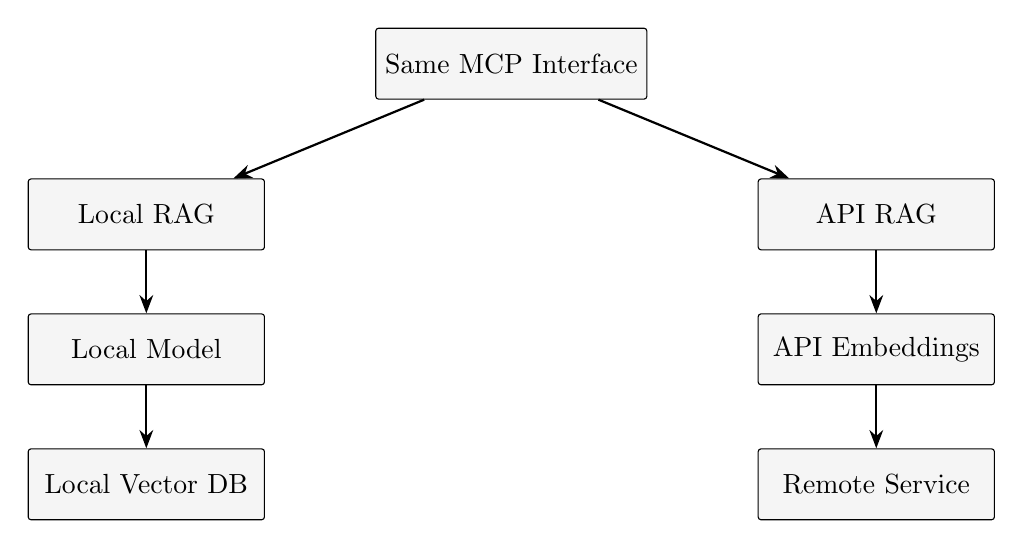
\begin{tikzpicture}[
    box/.style={draw, rounded corners=1pt, align=center,
                minimum width=30mm, minimum height=9mm, fill=gray!8},
    arr/.style={-{Stealth}, thick}
  ]
  \node[box] (iface) {Same MCP Interface};
  \node[box, below left=10mm and 14mm of iface] (local) {Local RAG};
  \node[box, below right=10mm and 14mm of iface] (api)   {API RAG};
  \node[box, below=8mm of local] (lmod) {Local Model};
  \node[box, below=8mm of api]   (amod) {API Embeddings};
  \node[box, below=8mm of lmod]  (lvdb) {Local Vector DB};
  \node[box, below=8mm of amod]  (avdb) {Remote Service};

  \draw[arr] (iface) -- (local);
  \draw[arr] (iface) -- (api);
  \draw[arr] (local) -- (lmod);
  \draw[arr] (lmod)  -- (lvdb);
  \draw[arr] (api)   -- (amod);
  \draw[arr] (amod)  -- (avdb);
\end{tikzpicture}
\caption{Local and API implementations expose equivalent retrieval capabilities behind the same MCP interface.}
\label{fig:comparison}
\end{figure}

The research question becomes: \emph{how does a fully local RAG implementation
perform compared with an API-dependent implementation when both expose
equivalent retrieval capabilities to an LLM?}

\section{Recommended Baseline Architecture}
\label{sec:architecture-baseline}

For the initial proof of concept, the recommended architecture is shown in
Figure~\ref{fig:baseline}. It should be considered a \textbf{baseline
experimental system}, not necessarily the final production architecture.

\begin{figure}[htbp]
\centering
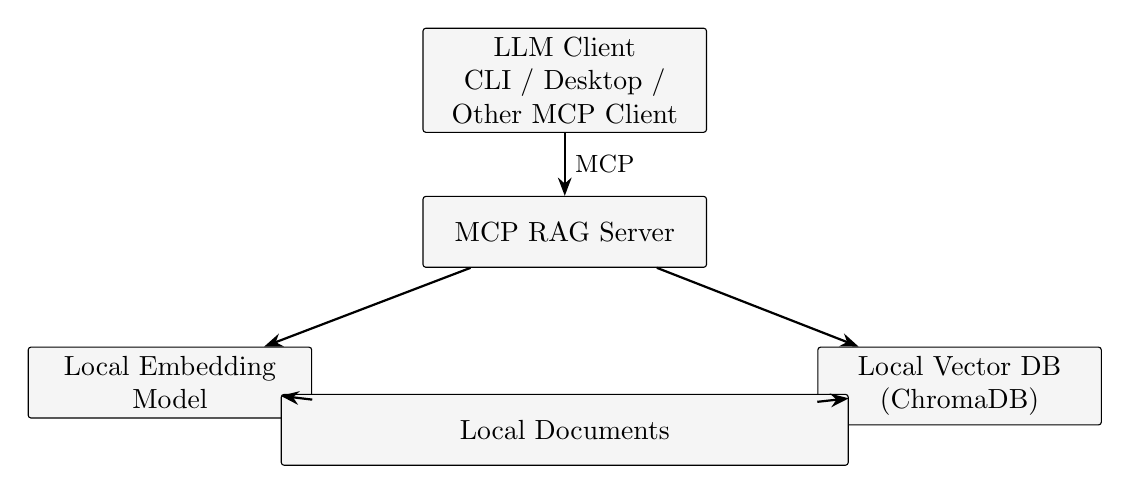
\begin{tikzpicture}[
    box/.style={draw, rounded corners=1pt, align=center,
                minimum width=36mm, minimum height=9mm, fill=gray!8},
    arr/.style={-{Stealth}, thick}
  ]
  \node[box] (client) {LLM Client\\CLI / Desktop /\\Other MCP Client};
  \node[box, below=8mm of client] (mcp) {MCP RAG Server};
  \node[box, below left=10mm and 14mm of mcp] (emb) {Local Embedding\\Model};
  \node[box, below right=10mm and 14mm of mcp] (vdb) {Local Vector DB\\(ChromaDB)};
  \node[box, below=16mm of mcp, minimum width=72mm] (docs) {Local Documents};

  \draw[arr] (client) -- node[right, font=\small] {MCP} (mcp);
  \draw[arr] (mcp) -- (emb);
  \draw[arr] (mcp) -- (vdb);
  \draw[arr] (emb) -- (docs);
  \draw[arr] (vdb) -- (docs);
\end{tikzpicture}
\caption{Recommended baseline architecture: MCP-based local RAG server.}
\label{fig:baseline}
\end{figure}

Its primary strengths are: clear separation of components; minimal
implementation complexity; local execution; a reusable tool interface;
compatibility with MCP-based clients; easy substitution of RAG components; and
strong suitability for controlled benchmarking.

\section{Conclusions: Three Ways to Implement a Local RAG}
\label{sec:conclusions}

The decision guide in Sections~\ref{sec:architecture} and~\ref{sec:infra}
converges on three viable ways to build a RAG system for regulatory and
technical documentation. They differ mainly in the trade-off between
\textbf{control} and \textbf{time-to-deployment}: the more ready-made the
solution, the faster it runs, but the less control it leaves over retrieval
quality. Each option is evaluated below in terms of hardware needed,
advantages, disadvantages, and target public.

\subsection{Option 1: Custom RAG + Local LLM or API}

The entire pipeline (ingestion, chunking, embeddings, vector database,
retrieval orchestration, and frontend) is built from scratch. Generation runs
on a local LLM or on a cloud API, according to the infrastructure decision in
Section~\ref{sec:infra}.

\textbf{Hardware needed.} Local inference requires a GPU (8--24~GB of VRAM or
more for models in the 7B--70B range) plus CPU, RAM, and disk for indexing
and the vector database. The API variant needs no GPU: only a workstation
with network access. In practice the 7B--70B range spans very different
tiers: 7B--8B models run comfortably on a single consumer GPU with
6--8~GB of VRAM, while 70B models need roughly 22~GB of VRAM even at
4-bit quantization and remain slow (single-digit tokens/second) on one
consumer card; usable 70B throughput typically requires 40~GB or more of
VRAM across multiple data-center-class GPUs \cite{localbench}.

\textbf{Advantages.} Total control over every stage of the pipeline; custom
user interface, analytics, and re-ranking; millisecond-level latency
optimization; no dependency on third-party clients. The API variant also
provides state-of-the-art reasoning.

\textbf{Disadvantages.} High technical debt; development cycles of months;
constant pipeline maintenance; ``reinventing the wheel'' for integrations.
The local variant is constrained by VRAM and by the reasoning capacity of
local models on complex legal or regulatory jargon.

\textbf{Target public.} Companies with AI-core products (e.g., B2B SaaS) and
teams that need their own frontend, analytics, or deep integration with
non-standard legacy systems.

\subsection{Option 2: Open-Source MCP RAG Software (Ready to Use)}

Existing ready-made MCP RAG servers package a local RAG system behind the
standard MCP interface with zero code. A representative example is
\texttt{mcp-local-rag} \cite{mcp-local-rag}: a local-first server with hybrid
keyword (BM25) + semantic search, launched with a single \texttt{npx}
command, configured by pointing a \texttt{BASE\_DIR} at the documents, and
consumable by any MCP client (Cursor, Claude Code, Codex, etc.).

\textbf{Hardware needed.} Minimal. Embeddings run on CPU by default
(all-MiniLM-L6-v2 on ONNX Runtime), storage is a file-based vector database
(LanceDB), and after the initial model download, ingestion and search work
fully offline. No API keys, Docker, Python, or external database are
required.

\textbf{Advantages.} Deployment in minutes or hours; no development effort;
standard MCP interface reusable across clients; full local privacy; hybrid
search quality out of the box.

\textbf{Disadvantages.} Limited control over chunking, embeddings, and
retrieval internals; retrieval quality is bounded by the tool's features and
default models; customization requires extending or forking third-party code;
roadmap and maintenance are owned by an external project.

\textbf{Target public.} Internal teams, law firms, and individual developers
who need fast, private document search integrated with their existing AI
clients, and teams that want to validate a corpus before committing to a
custom build.

\subsection{Option 3: Custom RAG Server via MCP with the Python SDK}

A custom MCP server is built with the official Python SDK \cite{mcp-sdk},
wrapping a local RAG pipeline (local embeddings + local vector database) and
exposing retrieval as MCP tools. This is the solution proposed and detailed
in Section~\ref{sec:solution}.

\textbf{Hardware needed.} Same profile as the local path of Option~1 minus
the LLM: embeddings run on CPU or optionally on GPU, and the index needs RAM
and disk. No GPU is strictly required for a prototype.

\textbf{Advantages.} Full control of retrieval quality behind a standardized
interface; separation of concerns; components (embedding model, vector
database) are independently substitutable; the server is benchmarkable as an
independent subsystem; reusable across any MCP-compatible client.

\textbf{Disadvantages.} Development and maintenance effort (small for a
prototype but real); MCP adds a process and communication layer; benefits
depend on the client tool's reasoning quality.

\textbf{Target public.} Research teams running controlled local-versus-API
experiments, developers who need to connect an LLM to internal documentation,
and organizations with sensitive documents that require control over the
retrieval pipeline.

\subsection{Comparison and Bottom Line}

Table~\ref{tab:options} summarizes the three options.

\begin{longtable}{>{\raggedright\arraybackslash}p{2.2cm}>{\raggedright\arraybackslash}p{4.2cm}>{\raggedright\arraybackslash}p{4.2cm}>{\raggedright\arraybackslash}p{4.2cm}}
\caption{Comparison of the three implementation options.}
\label{tab:options}\\
\toprule
\textbf{Attribute} & \textbf{Option 1: Custom RAG + Local LLM or API} & \textbf{Option 2: Open-Source MCP RAG Software} & \textbf{Option 3: Custom MCP RAG Server (Python SDK)} \\
\midrule
\endfirsthead
\toprule
\textbf{Attribute} & \textbf{Option 1: Custom RAG + Local LLM or API} & \textbf{Option 2: Open-Source MCP RAG Software} & \textbf{Option 3: Custom MCP RAG Server (Python SDK)} \\
\midrule
\endhead
Hardware needed &
\begin{itemize}[leftmargin=1.2em, nosep, topsep=0pt]
  \item Local: GPU (8--24~GB VRAM+) for the LLM; CPU/RAM/disk for indexing and vector DB.
  \item API: no GPU; workstation + network.
\end{itemize} &
\begin{itemize}[leftmargin=1.2em, nosep, topsep=0pt]
  \item CPU only (default ONNX Runtime).
  \item File-based vector DB (LanceDB).
  \item Offline after the first model download.
\end{itemize} &
\begin{itemize}[leftmargin=1.2em, nosep, topsep=0pt]
  \item CPU (optional GPU) for embeddings.
  \item RAM/disk for the index.
  \item No GPU required for a prototype.
\end{itemize} \\
Advantages &
\begin{itemize}[leftmargin=1.2em, nosep, topsep=0pt]
  \item Total control of every stage.
  \item Custom UI, analytics, re-ranking.
  \item Millisecond latency optimization.
  \item SOTA reasoning via API.
\end{itemize} &
\begin{itemize}[leftmargin=1.2em, nosep, topsep=0pt]
  \item Deployment in hours; zero code.
  \item Standard MCP interface.
  \item Fully local and private.
  \item Works with any MCP client.
\end{itemize} &
\begin{itemize}[leftmargin=1.2em, nosep, topsep=0pt]
  \item Full retrieval control + standard interface.
  \item Substitutable components.
  \item Independently measurable.
  \item Reusable across clients.
\end{itemize} \\
Disadvantages &
\begin{itemize}[leftmargin=1.2em, nosep, topsep=0pt]
  \item High technical debt.
  \item Months of development.
  \item Constant maintenance.
  \item VRAM and local model limits.
\end{itemize} &
\begin{itemize}[leftmargin=1.2em, nosep, topsep=0pt]
  \item No control over chunking, embeddings, retrieval internals.
  \item Quality bounded by the tool.
  \item Roadmap owned by a third party.
\end{itemize} &
\begin{itemize}[leftmargin=1.2em, nosep, topsep=0pt]
  \item Own development and maintenance.
  \item MCP adds a process/communication layer.
  \item Client-tool dependency.
\end{itemize} \\
Target public &
\begin{itemize}[leftmargin=1.2em, nosep, topsep=0pt]
  \item AI-core companies and B2B SaaS.
  \item Teams needing their own frontend and analytics.
\end{itemize} &
\begin{itemize}[leftmargin=1.2em, nosep, topsep=0pt]
  \item Internal teams, law firms, individual developers.
  \item Quick private search; corpus validation pilots.
\end{itemize} &
\begin{itemize}[leftmargin=1.2em, nosep, topsep=0pt]
  \item Research teams running local-vs-API experiments.
  \item Developers and organizations with sensitive documents.
\end{itemize} \\
\bottomrule
\end{longtable}

There is no single winner: the choice depends on whether the priority is
control (Option~1), speed of deployment (Option~2), or a balance of both
(Option~3). For this project, \textbf{Option~3 is the recommended baseline}:
it keeps the retrieval pipeline fully controllable and measurable while the
MCP interface provides the stable boundary required by the experimental
methodology of Section~\ref{sec:methodology}. Option~2 is the ideal pilot to
validate the document corpus in hours, and Option~1 remains the path for a
future product with its own user interface and analytics.

\begin{quote}
\emph{MCP for interoperability + local embeddings for privacy and independence
+ local vector storage for retrieval + a controlled benchmark for comparing
local and API-based implementations.}
\end{quote}

\begin{thebibliography}{13}

\bibitem{mcp-spec}
Model Context Protocol Specification (2026-07-28).
\url{https://github.com/modelcontextprotocol/modelcontextprotocol/blob/main/docs/specification/2026-07-28/server/tools.mdx}

\bibitem{mcp-sdk}
Official MCP Python SDK. The \texttt{main} branch README documents v1.x as the
current stable release; v2 is pre-alpha and under active development as of
August 2026.
\url{https://github.com/modelcontextprotocol/python-sdk}

\bibitem{rag-survey}
RAG Evaluation Survey (2026). SN Computer Science.
\url{https://link.springer.com/article/10.1007/s42979-026-05134-x}

\bibitem{docling}
Docling: Document ingestion and parsing.
\url{https://github.com/docling-project/docling}

\bibitem{ragas}
Es, S., James, J., Espinosa-Anke, L., Schockaert, S. (2024). RAGAS: Automated Evaluation of Retrieval Augmented Generation. EACL 2024.
\url{https://aclanthology.org/2024.eacl-demo.16/}

\bibitem{ragchecker}
RAGChecker: A Fine-grained Framework for Diagnosing RAG (2024). arXiv:2408.08067.
\url{https://arxiv.org/abs/2408.08067}

\bibitem{colpali}
ColPali: Efficient Document Retrieval with Vision Language Models (2024). arXiv:2407.01449.
\url{https://arxiv.org/abs/2407.01449}

\bibitem{mteb}
MTEB: Massive Text Embedding Benchmark.
\url{https://docs.mteb.org/overview/available_benchmarks/}

\bibitem{vdbbench}
Vector Database Benchmark (2026). Journal of Big Data and Artificial Intelligence.
\url{https://jbdai.org/index.php/JBDAI/article/view/80}

\bibitem{graphrag}
Microsoft Research. GraphRAG.
\url{https://www.microsoft.com/en-us/research/project/graphrag/overview/}

\bibitem{localbench}
Local Inference Benchmark (July 2026). Vendor-published benchmark (Plugsky);
figures are directionally useful but were not produced by an independent or
peer-reviewed source.
\url{https://plugsky.com/local-inference-benchmark}

\bibitem{ane-mintic}
ANE/MinTIC Regulatory Compilation (Colombia).
\url{https://normograma.mintic.gov.co/mintic/compilacion/cndstr_ane_agencia_nacional_espectro.html}

\bibitem{mcp-local-rag}
mcp-local-rag: Local-first RAG server for developers (MCP). MIT License.
\url{https://github.com/shinpr/mcp-local-rag}

\end{thebibliography}

\end{document}